\documentclass[12pt,preprint]{aastex}
% for \sout
\usepackage{ulem}
% makes sure \em{} is italic rather than underlined (corrects ulem from line above)
\normalem

% for the red MarginPars
\usepackage{color}

% some extra math symbols
\usepackage{mathtools}

\newcommand{\rhocutoff}{\rho_\mathrm{cutoff}}
\newcommand{\rhoanelastic}{\rho_\mathrm{anelastic}}

\newcommand{\gcc}{\mathrm{g~cm^{-3} }}
\newcommand{\Tcutoff}{T_\mathrm{cutoff}}

% MarginPars
\setlength{\marginparwidth}{0.75in}
\newcommand{\MarginPar}[1]{\marginpar{\vskip-\baselineskip\raggedright\tiny\sffamily\hrule\smallskip{\color{red}#1}\par\smallskip\hrule}}


\newcommand{\msolar}{\mathrm{M}_\odot}

\begin{document}

%==========================================================================
% Title
%==========================================================================
\title{Double White Dwarf Mergers with CASTRO\\ I. Methodology and Code Validation}

\shorttitle{DWD Mergers. I. Methodology}
\shortauthors{Max}

\author{TBD}
%==========================================================================
% Abstract
%==========================================================================
\begin{abstract}
Notes on WD mergers
\end{abstract}
\keywords{hydrodynamics - methods: numerical - nuclear reactions, 
          nucleosynthesis, abundances - supernovae: general - white dwarfs}

%==========================================================================
% Introduction
%==========================================================================
\section{Introduction}



%==========================================================================
% Numerical Methodology
%==========================================================================
\section{Numerical Methodology}\label{sec:Numerical Methodology}

We use the Castro code as described in \citet{castro}.  For all the runs,
the PPM reconstruction is done, using the original limiters \citep{ppm}.
The original implementation of the PPM prediction in Castro takes the
form:
\begin{equation}
q_{i+1/2,L}^{n+1/2} = q_i -
   \sum_{\nu;\lambda^{(\nu)}\ge 0} l^{(\nu)} \cdot \left [
        q_i - \mathcal{I}_+(\sigma_\nu)
       \right ] r^{(\nu)}
\end{equation}
where $q$ is the vector of primitive variables, with $q_i$
representing the average in the cell, $l$ and $r$ are the left and
right eigenvectors with eigenvalue $\lambda$.  The sum is over all the
waves that result from the characteristic structure of the problem,
but designed such that only waves moving toward the interface
contribute to the interface value, $q_{i+1/2,L}^{n+1/2}$.  Finally,
$\mathcal{I}_+(\sigma_\nu)$ is the jump carried to the right interface
of the cell by the wave $\nu$, constructed by averaging under the
parabolic interpolant in the cell all information that can reach the
interface over the timestep.  $\sigma$ here is the fraction of the
zone crossed by the wave denoted by $\nu$.  The reader is referred to
\citet{ppmunsplit} for further defaults.

The presence of $q_i$ in this expression serves as a reference state.
The idea is that the error in the characteristic projection of the
jump (due to the nonlinearity) is minimized if we pick a suitable
reference state, since we only care about the jumps carried to the
interface over the timestep.  The original Castro implementation used
the cell-average quantity.  Experiments found that this is ill-behaved
in the presence of strong shocks (especially at low resolution). For
the present work, we switch the reference state to the jump carried by the 
fastest wave moving toward the interface, $\mathcal{I}_+(\sigma_3)$ in this
case, where the $3$ here means the wave associated with the $u + c$ eigenvalue.
This is in agreement with \citet{ppmunsplit} (eq. 90).  This makes our
expression appear as:
\begin{equation}
q_{i+1/2,L}^{n+1/2} = \mathcal{I}_+(\sigma_3) -
   \sum_{\nu;\lambda^{(\nu)}\ge 0} l^{(\nu)} \cdot \left [
        \mathcal{I}_+(\sigma_3)  - \mathcal{I}_+(\sigma_\nu)
       \right ] r^{(\nu)}
\end{equation}




boundary conditions

initial models

AMR


%==========================================================================
% Test Problems
%==========================================================================
\section{Test Problems}\label{Sec:Tests}

\subsection{Maintaining Hydrostatic Equilibrium}\label{Sec:HSE}

\subsection{Gravitational Free Fall}\label{Sec:Gravitational Free Fall}

A simple test to verify the Poisson solver implemented by CASTRO is
the case of gravitational free fall. In this setup, two stars, each
individually in an equilibrium state, are placed on the computational
grid, separated by an initial distance $r_0$ along the $x$ axis with
zero initial velocity. We choose stars of masses $0.6$ and $0.8\,
M_\odot$, with the lower mass star on the left side (e.g. $x < 0$) of
the domain and the higher mass star on the right, such that their
center of mass coincides with the center of the
domain. Gravitationally, the stars may be treated as point masses
until the point of contact, so the equation of motion governing the
distance $r$ between their centers of mass is that of simple free
fall:
\begin{equation}
  \ddot{r}(t) = - \frac{GM}{r},
\end{equation}
where $G$ is the gravitational constant and $M$ is the total mass of
the system. This differential equation has a closed-form solution for
the evolution time as a function of separation:
\begin{equation}
  t(r) = \sqrt{\frac{r_0^3}{2GM}} \left[ \text{arccos}\left(\sqrt{\frac{r}{r_0}}\,\right) + \sqrt{\frac{r}{r_0} \left(1 - \frac{r}{r_0}\right)}\ \right]. \label{analyticalFreeFall}
\end{equation} \MarginPar{is there a reference for this? or did you derive it?}
We determine the initial separation to be consistent with the
simulation performed in Section \ref{Sec:Kepler}; that is, we select
an initial orbital period and use Kepler's third law to calculate the
radius of a circular orbit with that period. We select an initial
orbital period of 200 s for this simulation, so that the separation is
\[
  r_0 = 5.73 \times 10^{9}\ \text{cm}.
\]
We chose a relatively low resolution simulation to demonstrate the
capabilities of CASTRO even while using modest resources. The
computational grid is covered by a coarse grid of $48^3$ zones, with
two levels of refinement above the coarse grid. Each refined grid
carries an increase in resolution by a factor of 4 relative to the
coarser grid below it. CASTRO initially assigns $93\%$ of the domain
to be covered by the intermediate resolution grids, and $0.05\%$ of
the domain to be covered by the finest resolution grids.

The analytical result in Equation \ref{analyticalFreeFall} determines
the total elapsed free-fall time,
\[
  t_{\text{ff}} = \frac{\pi}{2} \sqrt{\frac{r_0^3}{2GM}}.
\]
The physical radius of each white dwarf is roughly $10\%$ of the
initial separation, so we consider the evolution terminated when the
radial separation reaches that value (at that point, the stars will no
longer be in free-fall due to physical contact). Since the elapsed
time goes roughly as the square root of the distance for small $r$, we
consider the evolution terminated when $t = 0.99\, t_{\text{ff}}$. The
results of our simulation are shown in Figure \ref{Fig:Free Fall}.

\begin{figure}
  \centering
  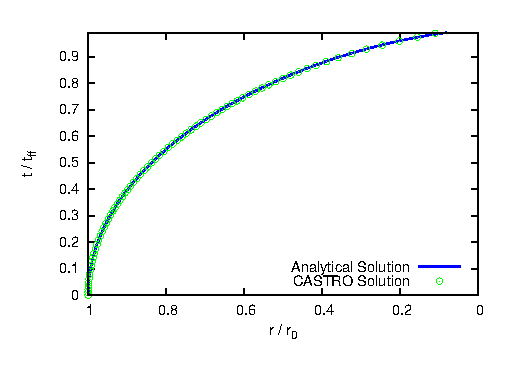
\includegraphics[scale=2.0]{freefall/plot_freefall}
  \caption{Time evolution of two initially stationary white dwarfs,
    mutually attracted to each other by the gravitational force. The
    horizontal axis gives the separation of the white dwarfs, scaled
    to the initial separation, and the vertical axis gives the elapsed
    time of the simulation, scaled to the total elapsed time
    necessarily. The solid curve shows the analytical result,
    calculated from Newtonian mechanics, and the circles show the
    samples from the time evolution with CASTRO. The agreement between
    theory and simulation is excellent, even for a simulation with
    modest resolution.}
  \label{Fig:Free Fall}
\end{figure}

\subsection{Keplerian Orbit}\label{Sec:Kepler}

%==========================================================================
% Conclusions
%==========================================================================
\section{Conclusions and Discussion}\label{Sec:Conclusions and Discussion}


\acknowledgments


\clearpage

\bibliographystyle{apj}
\bibliography{ws}

\end{document}

